\documentclass[a4paper,12pt,twoside]{report}
\usepackage{hyperref}
\usepackage{graphicx}
\usepackage{listings}
\usepackage{pdfpages}
\usepackage{color}
\usepackage{titlesec}
\usepackage{fancyhdr}
\pagestyle{fancy}
\renewcommand*\chaptermark[1]{\markboth{\thechapter. #1}{}}
\fancyhf{}
\fancyhead[LE,RO]{\thepage}
\fancyhead[LO,RE]{\leftmark}
\setlength{\headheight}{14.5pt}
\lstset{breaklines=true}
\lstset{basicstyle=\small\ttfamily}
\lstset{columns=fixed}
\definecolor{Brown}{cmyk}{0,0.81,1,0.60}
\definecolor{OliveGreen}{cmyk}{0.64,0,0.95,0.40}
\definecolor{CadetBlue}{cmyk}{0.62,0.57,0.23,0}
\lstset{language=XML,
  keywordstyle=\ttfamily\color{OliveGreen},
  identifierstyle=\ttfamily\color{CadetBlue}\bfseries,
  commentstyle=\color{Brown},
  stringstyle=\ttfamily,
  showstringspaces=true}

\raggedbottom

\let\tmp\oddsidemargin
\let\oddsidemargin\evensidemargin
\let\evensidemargin\tmp
\reversemarginpar

\titleformat{\chapter}[block]
{\normalfont\huge\bfseries}{\thechapter.}{1em}{\Huge}

\title{A real time train information and prediction system for the London Underground --- final report}
\author{Murray Colpman --- Supervisor: Nick Gibbins}
\begin{document}
\begin{titlepage}
  \begin{center}
    \textsc{\Large Electronics and Computer Science}\\
    \textsc{\Large Faculty of Physical Sciences and Engineering}\\
    \textsc{\Large University of Southampton}\\[1.5cm]
    \textsc{\Large Murray Colpman}\\
    \textsc{\Large \today}\\[1.5cm]
    \textsc{\LARGE A real time train information and prediction system for the London Underground}\\[1.5cm]
    \textsc{\large Project supervisor: Nick Gibbins}\\
    \textsc{\large Second examiner: Iain McNally}\\[1.5cm]
    \textsc{\large A project report submitted for the award of}\\
    \textsc{\large MEng Computer Science --- 4443}
  \end{center}
\end{titlepage}

\chapter*{Abstract}

The London Underground currently lacks publicly-available software allowing its
users to track individual trains through the system. This project addresses
this by creating a system to allow the user to view a list of trains due to
depart each station along with ones already departed, and to allow the user to
select a train to view its course throughout the system. This system includes
timetable inference, data collection and storage, and a web interface, and lays
the foundation for future systems that predict times based on actual
performance of trains, and produce maps of track codes (signalling blocks that
trains can occupy) based on the gathered data to further improve predictions.

\pagebreak

\tableofcontents

\pagebreak

\chapter*{Statement of Originality}

This is all my own work except where explicitly indicated otherwise, and except
for the ``static'' directory in the submitted code, which contains pre-packaged
software such as Twitter Bootstrap and Moment which I did not write, and the
``templates'' directory, the files in which were originally based on a Twitter
Bootstrap example template (heavily modified to produce the site). All sources
have been correctly acknowledged. 

My thanks go to Tom Cairns for providing the inspiration for this project with
Realtime Trains. Thanks also to my supervisor, Nick Gibbins; and second
examiner, Iain McNally; for their time and useful feedback.

\pagebreak

\chapter{Introduction}

The London Underground is a source of great interest for rail enthusiasts. With
its own rich history, there are occasional heritage operations such as the
recent Steam on the Met events organised by the London Transport Museum. Stock
withdrawal causes great interest in its own right, for example the desire to
ride on the last train of particular stock, or to ensure that you have ridden
on all trains before they are withdrawn. Finally, unique activities like the
Tube Challenge (visiting every London Underground station arriving or departing
by train in one day) also offer interest.

All of these tasks are currently hindered by the lack of a publicly-available
information system that allows the user to track trains through the network,
and yet the data required to create one is more or less available. This
project's aim was therefore to create such a system, allowing the user to view
the arrivals and departures in the near past, present and the future for a
given station, and also to track a given train through the system.

Such a system was primarily designed for rail enthusiasts. But as a byproduct
of producing the system, data has been collected which allowed a few inferences
to be made about the system. A small number of these have additionally been
explored.

The website Realtime Trains, developed by Tom Cairns, provides a similar system
for the National Rail network, on which the vast majority of heavy rail
services in Great Britain run. It makes use of open data provided by Network
Rail including schedules, amendments to schedules, details on trains passing
timing points, and details on the exact location of trains in the signalling
system.

Some similar data is available for the London Underground, from a system called
TrackerNet. However, there are a few important differences --- the system works
primarily on a pull, rather than a push, basis, so requests have to be
constantly made by the client. Due to this, results are cached for around
thirty seconds to prevent overloading TrackerNet. In addition to this, there is
no timetable data that can easily be cross-referenced with the live data,
except within a PDF which is not easily machine-readable. Finally, and in this
case in a similar manner to the Network Rail data, there is nothing to link the
signalling sections with physical location, neither topologically nor
geographically.

\section{Goals and scope}

\begin{enumerate}
  \item To produce a software system to track trains throughout the London
    Underground System and store the results of past days.
  \item To infer the working timetable for this data by averaging past runs.
  \item To produce a web-based user interface for viewing this data per-station
    or per-train.
  \item To expand the system to predict the future arrival and departure times
    of trains, including when forming new services. This is a stretch goal.
  \item To produce a topological map of track codes, and to use this map to
    further improve the predictions. This is a stretch goal.
\end{enumerate}

The main project comprises goals 1--3. Goals 4 and 5 are stretch goals.
Evaluation of the main project has been performed by testing a sample of the
produced timetable manually against the PDF and seeing how well they match.
Evaluation of goal 4 involves seeing how well the predictions match subsequent
reality. Evaluation of goal 5 is more difficult --- if a portion of a track
code map cannot be obtained, checking the map to ensure that at least the track
layout matches reality (maps of the London Underground track layout not
including signalling or track code data are commercially available from
TRACKmaps\cite{TRACKmaps5}) would be a reasonable evaluation step.

\section{Report summary}

Chapter 2 of this report contains background research on both the open data
available from London Underground Ltd and Network Rail, and on the state of
open data in general. The general state is improving but still quite poor, and
the London Underground is no exception to this. It has been generally
recognised what can be done to improve the situation, but the time and money
involved might prevent it from happening in the near future.

Chapter 3 lists the requirements of this system. These include a timetable
inference system based on observed train data gathered from TrackerNet, and a
way of viewing this data in a web interface.

Chapter 4 contains details on the design of the system, including the high
level design and more detail in specific areas.

Chapter 5 details the implementation of the system, including showing the final
structure of the software. It is written in Python using Flask for the web
interface with Twitter Bootstrap and JQuery.

Chapter 6 details both the tests performed on the software, and the evaluation
to test how well the software works in practice. Unit tests were written for
the timetable analysis code, and the timetables produced were generally
reasonably accurate.

Chapter 7 lists the project management techniques used and shows Gantt charts
for the project. The project took longer than expected, so the slack time in
which the stretch goals would have been attempted was instead taken by
completing the main goals on time.

Chapter 8 draws conclusions from the project and details what could be built on
it. The stretch goals represent the next logical step for the system, turning
it from a system primarily comprising groundwork but still useful for
enthusiasts, to a system more generally useful that can provide significant
insight into the network.

\chapter{Background}

Open transport data provides a useful source of information that could lead to
genuinely useful applications being produced, and yet in many cases it is left
untapped and mostly unused. This chapter explores why this might be the case by
summarising the state of open transport data, with particular focus on railways
including light rail and rapid transit systems like the London Underground. It
also details the state of the data from Network Rail and London Underground
Ltd, comparing the two to provide insight into why Network Rail's open data is
widely used for a variety of applications, and London Underground Ltd's is much
less well-used.

\section{Open transport data in the UK}

The recent Parliamentary Office of Science and Technology
briefing\cite{POSTnote472} states that the Department for Transport currently
publishes 255 datasets, of which 244 are issued under the Open Government
licence, which is a Creative Commons-compatible open data licence. However,
there are a further 481 datasets that are not currently published --- the vast
majority. It also states that data is frequently not retained or archived in
the sector. There is also the issue of the data being usable --- data that is
hard to use, or that is of questionable quality, will not encourage as much
usage as good quality and easy to use data. Fixing these issues may be
expensive and time-consuming, so there is a trade-off involved in opening up
data. It is worth noting that one user of Transport for London's London
Underground open data, the developer of Twitter bot @whensmytube, noted on his
blog that the London Underground open data is much more difficult to use and
less useful than the equivalent data for buses\cite{whensmytube}.

However, over-processing can also be a problem --- it has, for example, been
argued that raw data is often more useful than data pre-processed, perhaps
(intentionally or otherwise) with specific use cases in mind that sometimes
limit what can be done\cite{Robinson2009}. The wide variety of use cases of
open data should be kept in mind --- use cases for railway-related data can be
split into three broad categories\cite{Kuhn2011}: advanced search, to allow
users to search for specific attributes that may not be possible using the
operator's own website; mash-ups, which combine railway data with data from
other sources; and visualisations, for example a heat map of areas with most
delay, or a map showing where trains are physically located --- the latter of
which has been built for the London Underground using TrackerNet
data\cite{TrainTimesTube}.

Another survey, of accessibility data in particular, notes the difficulties of
relating data from multiple sources, and suggests publishing data as linked
open data to solve this\cite{Ding2014}.

There is also the issue that trains are operated commercially by multiple
companies, which causes data to be inconsistently available, or available but
not under open licences. For example, National Rail Enquiries (a part of the
Association of Train Operating Companies (ATOC), an association of all
passenger operators on the national network) until recently charged to access
their data. They now provide free access to individuals and small
organisations, but still charge a considerable fee for sites which have more
than five million usages in a four week period, meaning it is not true open
data. This data is the only source of some information on the National Rail
network such as delay causes and certain methods for train
cancellation\cite{CairnsSeminar2013}.


\section{Open data from Network Rail}

Rail enthusiasts make use of a website called Realtime Trains. For the National
Rail network, on which the vast majority of heavy rail services in Great
Britain run, this website makes use of open data mainly from four sources
provided by Network Rail (the public body that owns and maintains the
infrastructure and operates signalling equipment for nearly all of the
network)\cite{RTTData}:

\begin{itemize}
  \item TRUST, providing push data about trains passing certain timing points
    (mostly stations and junctions)
  \item TD, push data providing the train describer berth (which corresponds to
    a signalling section) that a given train is occupying --- cross-referenced
    with TRUST data to give more accurate predictions and platform alterations
  \item Schedule, pull data providing timetables for passenger and freight
    trains including changes to usual services (for engineering works, for
    example)
  \item VSTP, push data providing very short notice alterations to schedules
\end{itemize}

Realtime Trains uses these data sources to give views for the general public to
let people know where their train is, and to predict arrival times. It also has
a detailed view, allowing enthusiasts to see non-passenger trains, trains not
booked to stop at the station, detailed information about the routes trains are
booked to take (and actually take), and more detailed timing points. This can
be used by enthusiasts to track the position of a train they're interested in,
or just to see if any interesting trains are passing through a station.

\section{Open data from London Underground Ltd}

The London Underground, despite having a few areas of overlapping operation, is
not generally a part of the National Rail network, and so Realtime Trains does
not allow you to view information for the vast majority of its 270 stations.

Although the London Underground has an information system geared towards the
general public, there is currently no publicly-available software to track
individual trains through the system, nor is there a way to view the timetable
(both planned and predicted) from each station more than a few trains in
advance. Only ``live departure board'' style sites are available, showing for
each station when the next trains are due.

Such a tracking system would not only be useful for rail enthusiasts, for
example trying to follow a delayed steam service around the network or to
follow a particular train of interest, but would also be very useful for making
a variety of inferences about the network.

The main source of open data comes from a system called TrackerNet. TrackerNet
is a pull-based system, so a request must be made by the client every time new
data is desired. Data is requested over HTTP and returned in an XML format. To
prevent flooding, this data is cached for around thirty seconds (though in
reality, caching up to a minute is common).

There are four main endpoints available when using this data --- LineStatus
which returns overview information about the operation of each line (whether
there is disruption or closures), StationStatus which gives similar information
about stations, PredictionSummary which gives basic train prediction
information on a per-line basis, and PredictionDetailed which gives more
detailed train prediction information. This is requested on a per-station and
per-line basis\cite{TrackerNetSpec}. Therefore, one request per station desired
for each line is required per half minute. When this report refers to
TrackerNet, unless otherwise stated the PredictionDetailed endpoint is meant.
An example of the data from the four PredictionDetailed endpoints can be found
in Appendix A.

This data contains an attribute called TrackCode, which is the most accurate
source of location data --- it represents the current signalling block in which
the train is located. However, there is no publicly-available data to represent
the location of track codes, neither geographical nor topological. The caching
of data and the fact that some track codes are quite short (less than 30
seconds apart) means that it is less than trivial to construct such a map.

There is another source of data --- the public timetable as used by the
Transport for London journey planner. It is stored in a format known as
TransXChange, a format developed as a national standard for storing UK bus
timetables\cite{TransXChangeSpec}. Unfortunately, this data does not receive
any supplements for engineering works or alterations to the usual timetable. It
also doesn't contain non-passenger trains, like empty workings or engineering
trains, which would be important to enthusiasts. Finally and crucially, there
does not appear to be a way to relate this data with the live data.

There are also PDF working timetables available\cite{TfLWTT}, which do contain
all trains and do contain IDs which can be cross-referenced with the live data
--- a set number, representing one particular train's workings throughout the
day; and a trip number, which increments each time the train terminates and
forms a new working.

\chapter{Requirements}

These requirements were made with producing a base system in mind, a system
that while still being useful in its own right, would primarily provide the
groundwork for future systems to infer more useful data about the system. As
such, they were designed to produce a system with a reasonable user interface
and one that could be run on common server configurations.

\section{Functional}

\begin{enumerate}
  \item The system should constantly gather data from TrackerNet about train
    locations. (Goal 1)
  \item The system should save this data into a database. (Goal 1)
  \item The system should convert the observations of the positions of trains
    to train arrival and departure times for each station and save these into
    the database. (Goal 1)
  \item The system should, given a reasonable quantity of data collected, be
    able to calculate a likely working timetable from the arrival and departure
    data and save this into the database. (Goal 2)
  \item The system should have a web-based user interface. (Goal 3)
  \item This interface should have a station view, allowing stations to be
    searched for and all the trains arriving/departing that station, both in
    the working timetable and in observed reality, displayed. (Goal 3)
  \item This interface should also have a train view, allowing all the stops
    for a given train to be viewed, both in the working timetable and in
    reality. (Goal 3)
\end{enumerate}

\section{Nonfunctional}

\begin{enumerate}
  \item The system should run on a typical Linux server, and not require an X
    server.
  \item The system should be able to collect data fast enough so as not to miss
    any significant data.
  \item The system should be fast enough for the web interface to be usable.
  \item The system should be designed with future expansion in mind,
    particularly with regards to the goals of producing a train prediction
    system and of producing a map of Track Codes.
\end{enumerate}

\chapter{Design}

The system should consist of multiple parts. The first part is the data
gatherer, which should gather data on given lines and stations from TrackerNet
and store it in a database. As much data as may be useful for future systems
should be recorded. At this stage, observations on trains should also be
translated into arrival and departure times. Then, in another part of the
system, a timetable should be inferred and stored in the database, by taking
the median of train arrival and departure times and the mode of other data.
These timetables should be split up based on weekdays, Saturdays and Sundays.
Finally, a web interface will allow display and searching of this data.

Using three separate entry points rather than a single monolithic piece of
software is simpler and adds flexibility --- allowing, for example, the data
gatherer to be run on multiple servers, and the interface to be run on a
different one still. For this reason, this solution also provides added
scalability.

\section{Algorithms}

There are a few simple algorithms required for this project, most notably in
the timetable analyser module.

This algorithm is used to calculate the values to go into an arrival/departure
record, based on observed movements. It first handles the case where there is
not already an existing arrival/departure object for this train on this date.
In this case, it simply sets the arrival time to the observed time plus
TrackerNet's predicted number of seconds to the station, and the departure time
to that plus a fixed dwell time.

It then handles the case where there was a previous entry, and the current
entry shows the train stopped at a station. If the new observation doesn't
contradict previous predictions, the previous predictions are kept because it
is not possible to determine how long the train has already been at the station
and how long it will be. However, if the new data contradicts previous data, so
the train is observed at the station before the previous predicted arrival
time, or after the previous predicted departure time, it sets the arrival and
departure times to the observed time, as a better estimate than the previous
one.

It finally handles the case where there was a previous entry and the current
entry shows a train not stopped at a station. In this case, the new data is
used due to its being more up-to-date, and the old simply discarded.

\begin{lstlisting}
IF NOT arrDepRecordExists(train):
  arrTime = train.whenCreated + train.secondsTo
  depTime = arrTime + dwellTime # dwellTime 20 secs for Victoria line
ELSE:
  result = getPreviousRecord(train)
  oldArrTime = result.arrTime
  oldDepTime = result.depTime
  IF train.secondsTo == 0:
    IF train.whenCreated < oldArrTime:
      arrTime = train.whenCreated # train arrived early
    ELSE:
      arrTime = oldArrTime # train (probably) arrived when expected
    IF train.whenCreated > oldDepTime: # train has not left when expected
      depTime = train.whenCreated
    ELSE:
      depTime = oldDepTime
  ELSE:
    arrTime = train.whenCreated + train.secondsTo
    depTime = arrTime + dwellTime
addArrDepRecordToDb(train, arrTime, depTime)
\end{lstlisting}

This algorithm is used to calculate the details to go into the timetable
database table, containing the inferred timetable. In particular, it uses a
simple median on times (ignoring dates), and a mode on the rest of the data.
Median seems the most accurate option, as mean will be thrown off by outliers
and mode is not suitable for continuous data like time.

\begin{lstlisting}
FUNC median(array, attribute):
  results = SORT(array, lambda x: x[attribute].toTime())
  IF results.length < 1:
    RETURN NULL
  IF results.length MOD 2 == 1:
    RETURN results[(results.length - 1) / 2][attribute].toTime()
  IF results.length MOD 2 == 0:
    RETURN (results[(results.length - 1) / 2][attribute].toTime() +
            results[(results.length) / 2][attribute].toTime()) / 2

FUNC mode(array, attribute):
  return most\_common(map(array, lambda x: x[attribute]))

FUNC calculateMedianFromTrainArrDeps(results, days):
  results = [results WHERE result.day IN days]

  arrMedian = median(results, "arrTime")
  depMedian = median(results, "depTime")
  IF arrMedian NULL or depMedian NULL:
    RETURN (NULL, NULL, NULL, NULL, NULL)
  destMode = mode(results, "destination")
  destCodeMode = mode(results, "destCode")
  platNoMode = mode(results, "platformNumber")

  return (arrMedian, depMedian, destMode, destCodeMode, platNoMode)
\end{lstlisting}

\section{Database}

There are multiple options for both the database engine and for the structure
of the database. For the database engine, the main choices are traditional
relational SQL-based databases such as MySQL, MariaDB and PostgreSQL; and
modern NoSQL databases that eschew the relational model in favour of others,
such as MongoDB which uses a document model.

Based on my prior knowledge combined with a little research, I determined that
NoSQL databases are generally more useful when storing data which is only
loosely structured or needs to be easily extensible. Since the data being
stored does not meet these criteria, I quickly decided on a relational
database.

For structuring the data in the database, there are also multiple approaches.
The most obvious approach is in a similar structure to the TrackerNet XML ---
stations have platforms which have trains in various states of approach at
different times. Trains could alternatively be linked specifically to locations
such as track codes as opposed to the requested station, but this could prove
troublesome since I have seen the occasional train in the data which had an
empty string for the track code.

There is also the possibility of tailoring the data for specific purposes ---
for example pre-calculating parts of averages of arrival times so that
relatively little database access would be needed to calculate the inferred
timetable, or storing the same data multiple times in different structures
entirely for different purposes. The latter of these would be useful for
storing things such as the inferred timetable and actual arrival/departure
times calculated from observations, such that the expensive task of
recalculating upon each access need not be performed.

Storing data in its rawest form seems most useful, especially since it is
always possible to incorporate aspects of the other ideas above should
calculations prove too slow in practice. As mentioned above, separate tables
are also used for storage of train arrivals and departures, and for inferred
timetables. However, some irrelevant, broken or not implemented data should not
be saved to the database.

Therefore, there are five main tables:
\begin{itemize}
  \item stations --- one entry per station per line. This table is used to
    store general information about stations, including the name of the station
    and the name of the line on which this particular entry is located.
  \item platforms --- one entry per station platform. This table is used to
    provide a human-readable description of the function of each platform, as
    well as the frontmost track code associated with it.
  \item trains --- one entry per train per caching time, for each platform.
    This table is structurally based on the TrackerNet data, and contains
    ``observations'' about trains from the point of view of a station ---
    specifically, their location at each update, and existing time predictions
    to the nearest second of the arrival at the given station. It also contains
    the set number and trip number, which uniquely identify a train on a given
    day, and various other information such as its destination.
  \item trainsArrDep --- one entry per train per station used by that train.
    This table contains similar data to ``trains'' (above), but converted from
    observations about trains to the much more useful arrival and departure
    times (based on adding the time of observation to the predicted seconds to
    arrival, and this plus a dwell time for departures).
  \item timetables --- one entry per train, generalised for a day. Separate
    entries for weekdays, Saturdays and Sundays. This table contains similar
    data to the above, but generalised for each day (of weekdays, Saturdays and
    Sundays) based on the inferred timetable.
\end{itemize}

\begin{figure}[h]
  \centering
  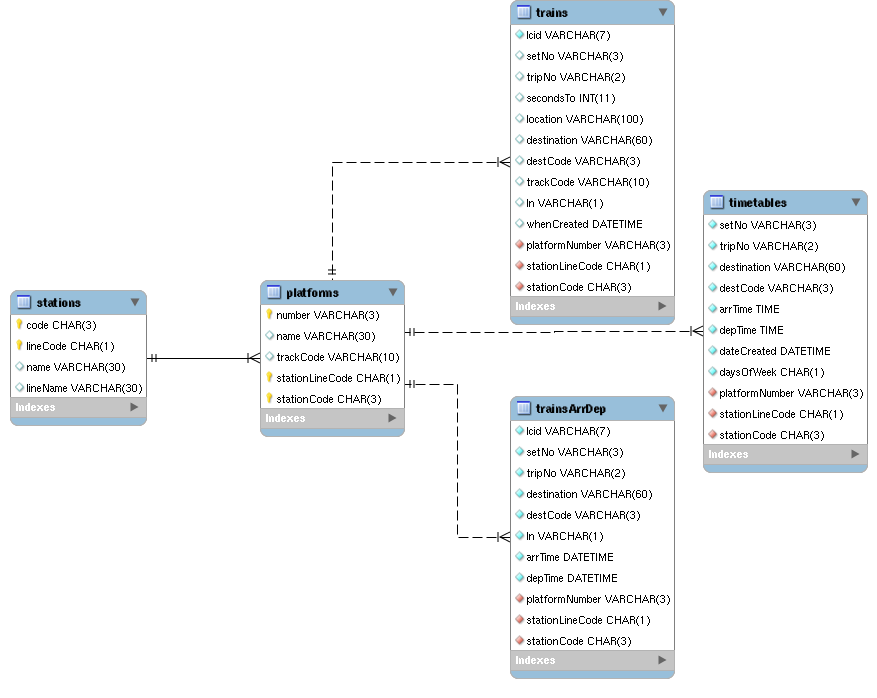
\includegraphics[width=\linewidth]{erd}
  \caption{Entity Relationship Diagram for database structure}
  \label{fig:erd}
\end{figure}

\section{Client-side website}

Since this project is mostly geared towards the backend than the frontend, I
need a simple web client that requires little set up and does not do much
client-side scripting, but still looks good. For this purpose, Twitter
Bootstrap, with which I am familiar at least in passing, is a reasonable
framework to use. There are other more complex frameworks available, but since
I am not particularly familiar with client-side web development, Twitter
Bootstrap is probably the easiest option here.

As for the look of the page, the most intuitive design is to have a search page
for stations, time periods and other filters; a results page for a single
station's trains for the time period specified and filtered using the given
filters; and a page for a single train's locations (past, present and future).
No alternative designs come to mind for this, and this design matches that of
most similar sites such as Realtime Trains, Open Train Times and National Rail
Enquiries.

URLs will be structured as follows:

/station/lineCode/stationCode/year/month/day/time --- station page

/train/lineCode/trainNo/tripNo/year/month/day/time --- train page

On the station page, each train listed will be a link to the respective train
page. Trains will be ordered in terms of actual departure and arrival times,
then if that doesn't exist by predicted departure and arrival times. The
station page will include search filters, at least by station name, line and
date/time (selectable with a calendar widget).

On the train page, stations will be listed in the order at which they were/will
be called. Each station will be a link to the station page showing other trains
around that time. There will also be a list of detailed information about that
train at the top.

The homepage can simply be the station page, but with a description of the site
replacing the results. This allows for quick access to the main feature of the
site --- the search.

\begin{figure}[h]
  \centering
  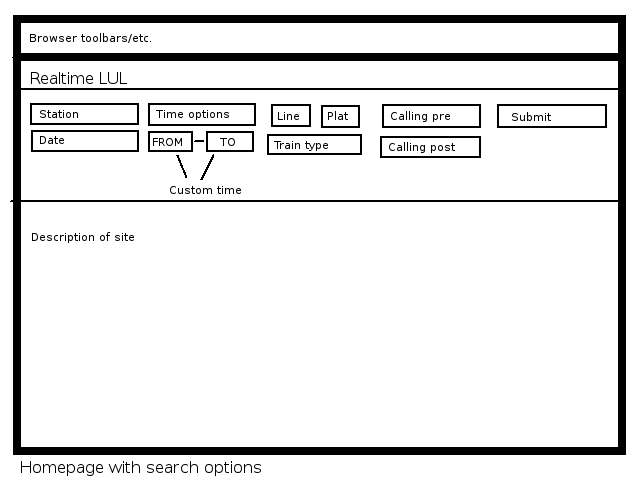
\includegraphics[width=\linewidth]{screen1}
  \caption{Diagrams of front page layout}
  \label{fig:screen1}
\end{figure}
\begin{figure}[h]
  \centering
  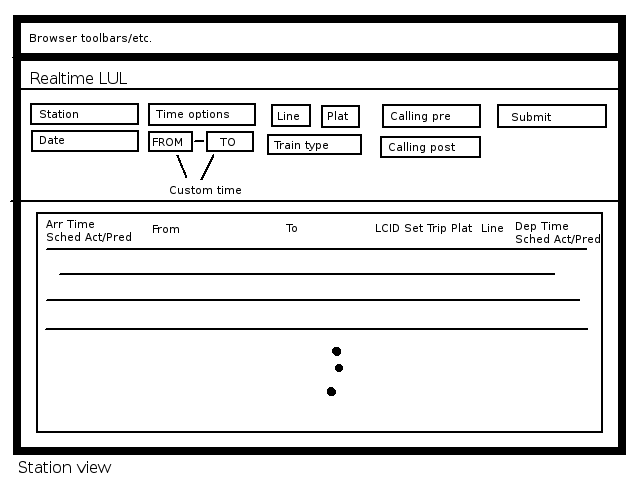
\includegraphics[width=\linewidth]{screen2}
  \caption{Diagram of station page layout}
  \label{fig:screen2}
\end{figure}
\begin{figure}[h]
  \centering
  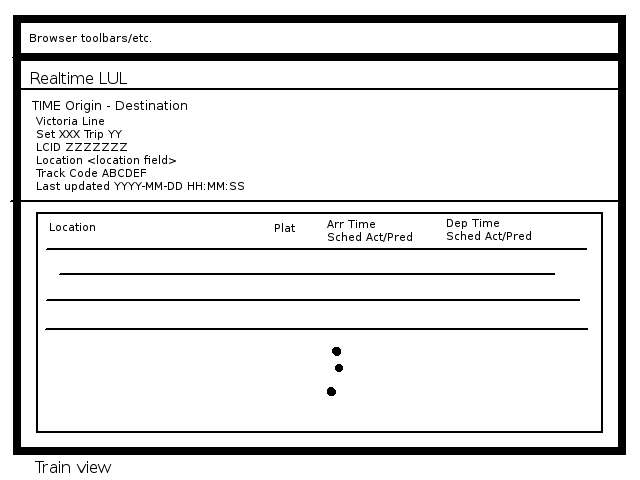
\includegraphics[width=\linewidth]{screen3}
  \caption{Diagram of train page layout}
  \label{fig:screen3}
\end{figure}

\chapter{Implementation}

The implementation took 1357 lines of Python, with 290 lines of HTML templates
and some miscellaneous JavaScript and CSS libraries not written by me as well.

All code was run through pylint. Due to differing naming conventions among
other things, full pylint compliance was not practical, but where possible
modifications were made to improve compliance.

The implementation was left deliberately line-agnostic, but most development
concentrated on using data from the Victoria line. This is because with a
limited computer and network connection on which to run the software, I had to
concentrate on just one line. The Victoria line is simpler with fewer edge
cases, so is more suitable as a starting point than some others.

Object orientation is used sparingly, only where it adds to simplicity. This is
most useful for code relating to the data logger, as it involves taking data
from one highly structured source and sending it to another, with some
processing. Storing this data as objects for manipulation purposes makes sense
here. However, for the web interface, where data from disparate sources needs
to be combined, often with missing fields, I found Python dicts to be a more
appropriate and flexible method of storage. In addition, Flask handles these
natively.

\section{Language choice}

The programming language in which the program is to be written is important. A
good choice in language can make a project easy to build and maintain and
increase reliability, whereas a poor choice can do just the opposite. I have
excluded obviously unsuitable languages, and languages in which I have little
experience.

Java is an obvious contender, being ubiquitous and versatile. However, it has
two important drawbacks --- it is not particularly suited for server-side web
development, and it is hard to get things done quickly, requiring a lot of
boilerplate code.

PHP is a popular choice for server-side web code, and would probably have
library support for everything that I might need to do. The main drawback is
that the design of the language is so poor that in my personal opinion too much
time is spent during development finding and fixing bugs that simply wouldn't
exist in most other languages.

Finally, Python is a mature language strongly suited to web development with a
large selection of libraries available. Getting things done is easy, but at the
expense of things like static typing which can lead to bugs or make debugging
harder. However, the design of the language is generally sound, certainly
moreso than JavaScript or PHP. It also has the issue that still not all
libraries are compatible with Python 3, which is the sensible choice for new
developments. However, despite these minor drawbacks, it is still, in my
opinion, the best language for this particular job, so I will be using it for
all server-side design.

Flask is the obvious choice for web development in Python, since it is
lightweight and easy to use, and powerful enough for this purpose.

\begin{figure}[h]
  \centering
  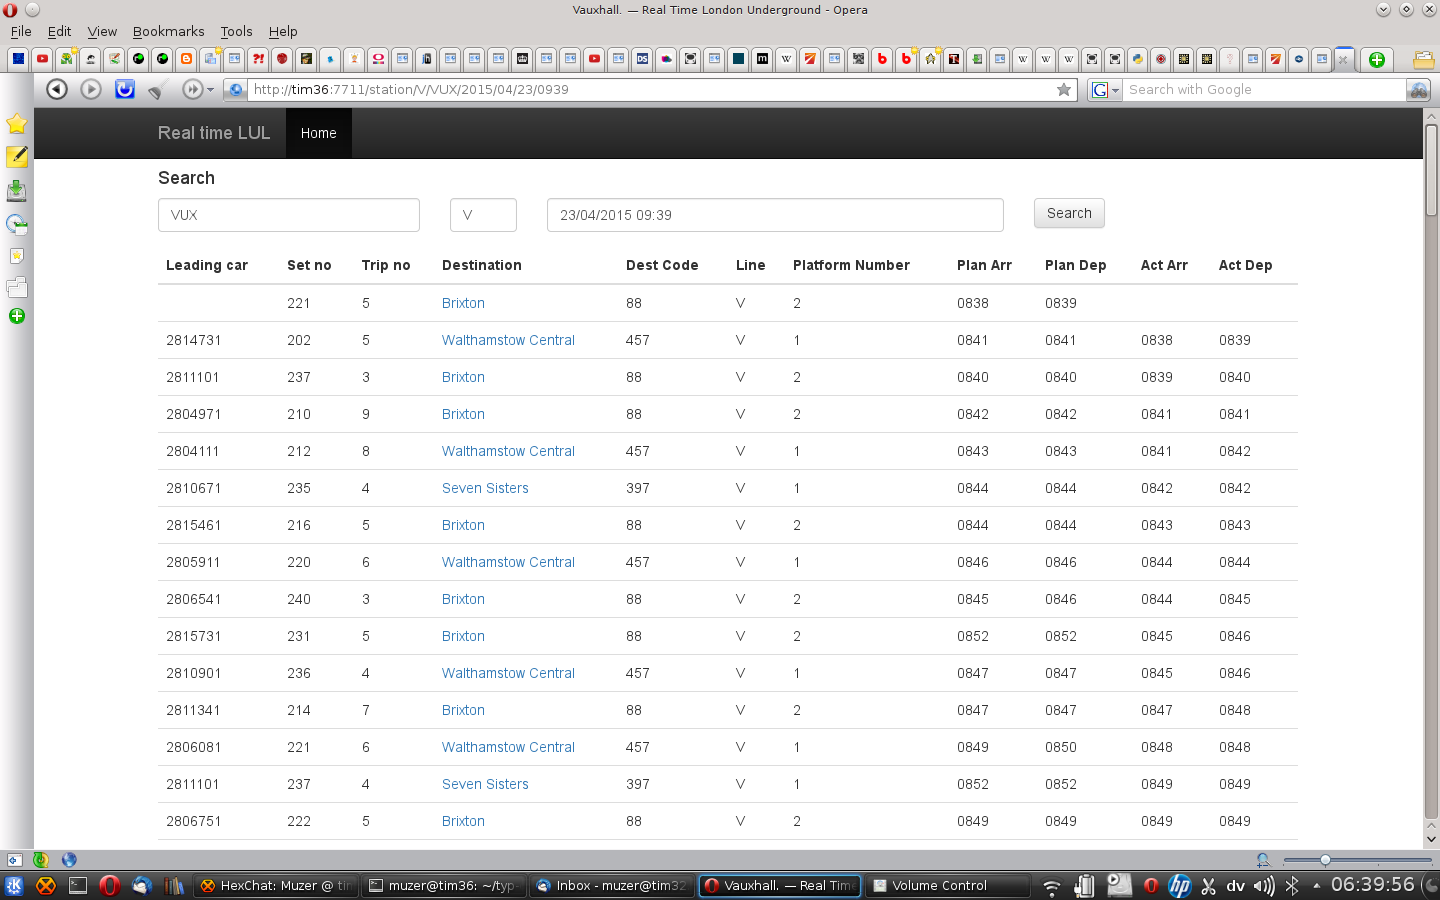
\includegraphics[width=\linewidth]{sshot1}
  \caption{Station page example}
  \label{fig:sshot1}
\end{figure}

\begin{figure}[h]
  \centering
  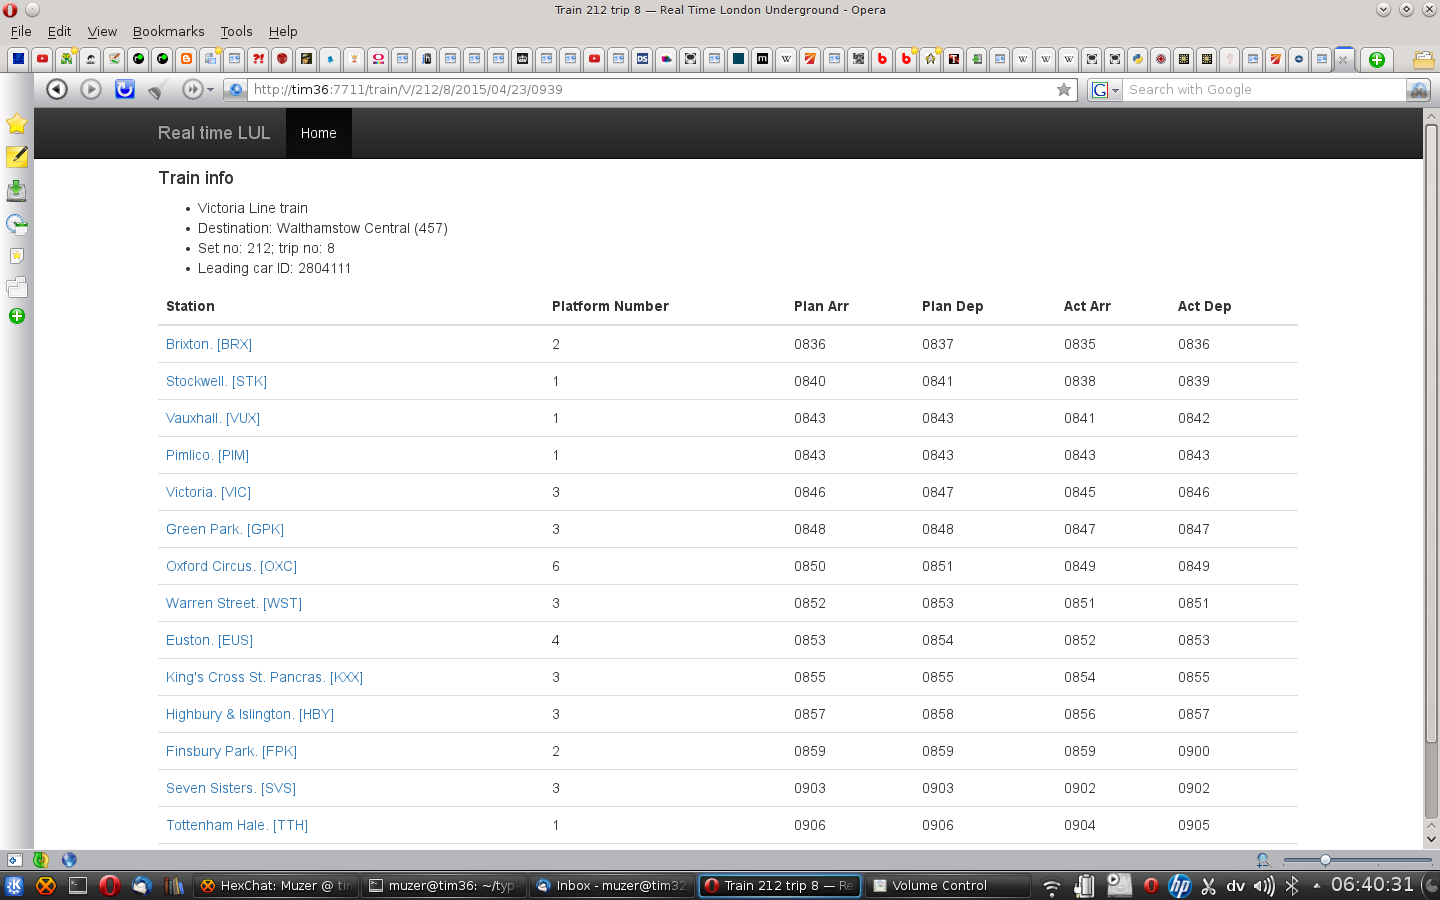
\includegraphics[width=\linewidth]{sshot2}
  \caption{Train page example}
  \label{fig:sshot2}
\end{figure}

\section{Module structure}

The software's overall design consists of a number of modules, a few of which
are entry points (ie executable in their own right). This is based on the
general structure required for the software itself --- not monolithic, but
instead a number of distinct tools sharing common code.

List of modules:
\begin{itemize}
  \item \texttt{data\_logger}: Entry point for the data logger. Execute it to
    start collecting data from TrackerNet and storing in database.
  \item \texttt{database\_access}: Provides functions to manipulate the
    database.
  \item \texttt{generate\_wtt}: Entry point for timetable inference. Execute it
    to generate a working timetable from the collected data.
  \item \texttt{linedefs}: Contains definitions for all the stations on each
    line, used for gathering data.
  \item \texttt{station}: Contains class definitions for station, platform and
    train classes.
  \item \texttt{timetable\_analyser}: Contains various functions to do with
    analysis of trains and timetable data.
  \item \texttt{timetable\_example}: Entry point for example usage of the
    timetable inference. Calculates a median for one particular example train.
  \item \texttt{trackernet\_access}: Contains functions to get data from
    TrackerNet.
  \item \texttt{ui}: Entry point for web interface. Runs a development server
    when executed.
\end{itemize}

\section{Tools}

Git was used for version control, with a private GitHub repository. Pylint and
Python's built in unit test functionality were also used to aid development.

\chapter{Testing and evaluation}

This project requires testing, to ensure that the code does what it was written
to do, and evaluation, to ensure that the end results are reasonably accurate.

\section{Testing}

\subsection{Unit testing}

Due to the nature of the project (accessing many external systems that are hard
to control or mock), unit testing has proven quite difficult. However, unit
tests have been written for the timetable analyser module, testing
comprehensively all functions that are used elsewhere. These functions were
written with unit testing in mind, with harder to simulate functionality like
database access split into wrapper functions for simplicity.

The calculation of train arrival and departure times was tested for all
possible code paths --- no previous entry, previous entry existing but where
train had arrived at a station earlier than that one predicted, previous entry
existing but where train had been observed at a station later than that one
predicted, previous entry existing where train arrived at a station but nothing
contradictory was observed, and train not arrived at a station but a previous
entry existing.

Unit tests were written for the brief functions to convert a datetime.time to
seconds and back. Finally, unit tests were written to fully test the median and
mode functions, and to test the function that used these to calculate a
timetable entry.

All tests pass. The tests themselves can be found in the design archive.

\subsection{Integration testing}

A brief testing plan was also drawn up to determine most likely points of
failure that need testing. In summary:

\begin{itemize}
  \item Searching for trains at various types of station, including Seven
    Sisters (at which some trains terminate), Brixton and Walthamstow Central,
    along with more usual intermediate stations. This is to ensure that termini
    work acceptably well in the interface. Many tweaks were performed as a
    result of this testing, including adding "Not In Service" as a special case
    where a train should be treated as being the same train as one previously
    in service, to ensure that a train wouldn't disappear as soon as it
    terminated without leaving behind arrival/departure times at the terminus.
  \item Testing around midnight. This brought up quite a few bugs that needed
    fixing, mostly involving database queries with time and date ranges.
    Searching for trains at midnight exactly, and clicking on an actual train
    that passed through midnight, all had to be tested.
  \item Testing various combinations of case and substrings in the station/line
    search functionality. All of these tests succeeded.
  \item Ensuring that all three cases of trains are tested --- ones with real
    running but no timetable, ones with timetable but not real running, and
    ones with both.
  \item Ensuring the screen is still readable when shrunk down to mobile size.
\end{itemize}

\section{Evaluation}

As mentioned in the scope definition, the main source of evaluation is by
manually comparing a sample of the generated timetable with the actual (PDF)
timetable, to see how well they match up. Therefore, I picked five trains at
random to perform this testing. The figure of five was chosen as manually
copying out and comparing the timetable is a slow process, and limited time was
available. I thought that I could provide a representative sample of at least
some of the different common cases with five. With five stations, I have 74
data points of departure times (though obviously some are linked to others),
which helps add to the significance of the evaluation. A list can be found in
Appendix B. In summary, aside from one outlier with a 28 minute difference,
timetable data was never more than 5 minutes out from the real timetable, and
the average error minutes per station were less than 1 for three out of five
trains.

The largest errors have often occurred on terminus stations, or those with
large waits. In some cases this cannot be helped, but in others it might be
possible to mitigate against some of these errors. For example, in the data 
used in the evaluation there is an error of 28 minutes. As far as I can tell,
this is most likely either from erroneous data, or from the train rarely
appearing for long enough at Brixton before moving on to another location to
show up on in the data logger, thus massively skewing the data towards times
when the train might show up, like times of disruption. Perhaps in these cases,
basing the departure data partially on a previous working would help.

Although valid timetables have shown to be quite accurate, while browsing the
site I have occasionally noticed anomalies like timetables for trains that
don't exist, and were (perhaps) caused by erroneous data. For example, train
255 trip 1 on weekdays appears to run from 0520 from Walthamstow Central up to
1228 at Brixton, which is obviously unfeasible. More heuristics to decide which
trains are likely to be real would fix this --- eliminating from the timetable
ones with only a few ``source'' trains compared to other trains, for example.

The project has largely satisfied the requirements. It collects data from
TrackerNet, stores it in a database, and calculates train arrival and departure
times from this. It calculates an inferred timetable that has a reasonable
level of accuracy (though this aspect could be further improved), and has a web
interface to view both the timetabled and actual arrival and departure times,
as well as other details about trains. It runs on a Linux server without X,
runs reasonably fast even with a big database, and is designed with expansion
in mind.

The tests show that the project functions on a technical level, and the success
of the timetable evaluation shows that the project is able to function on a
realistic and practical level as well, given more time to iron out the
remaining flaws and more data collected.

\chapter{Project management}

The project started running behind schedule during the actual implementation,
so the slack time available in which I would have attempted to carry out the
stretch goals was instead taken up by the main goals, due in part to a higher
than expected workload this semester. The final project was, however, submitted
on time and to the originally-intended scope.

Git was used for version control of source code and of reports.

The first Gantt chart shows the planned work; the second shows the actual work.

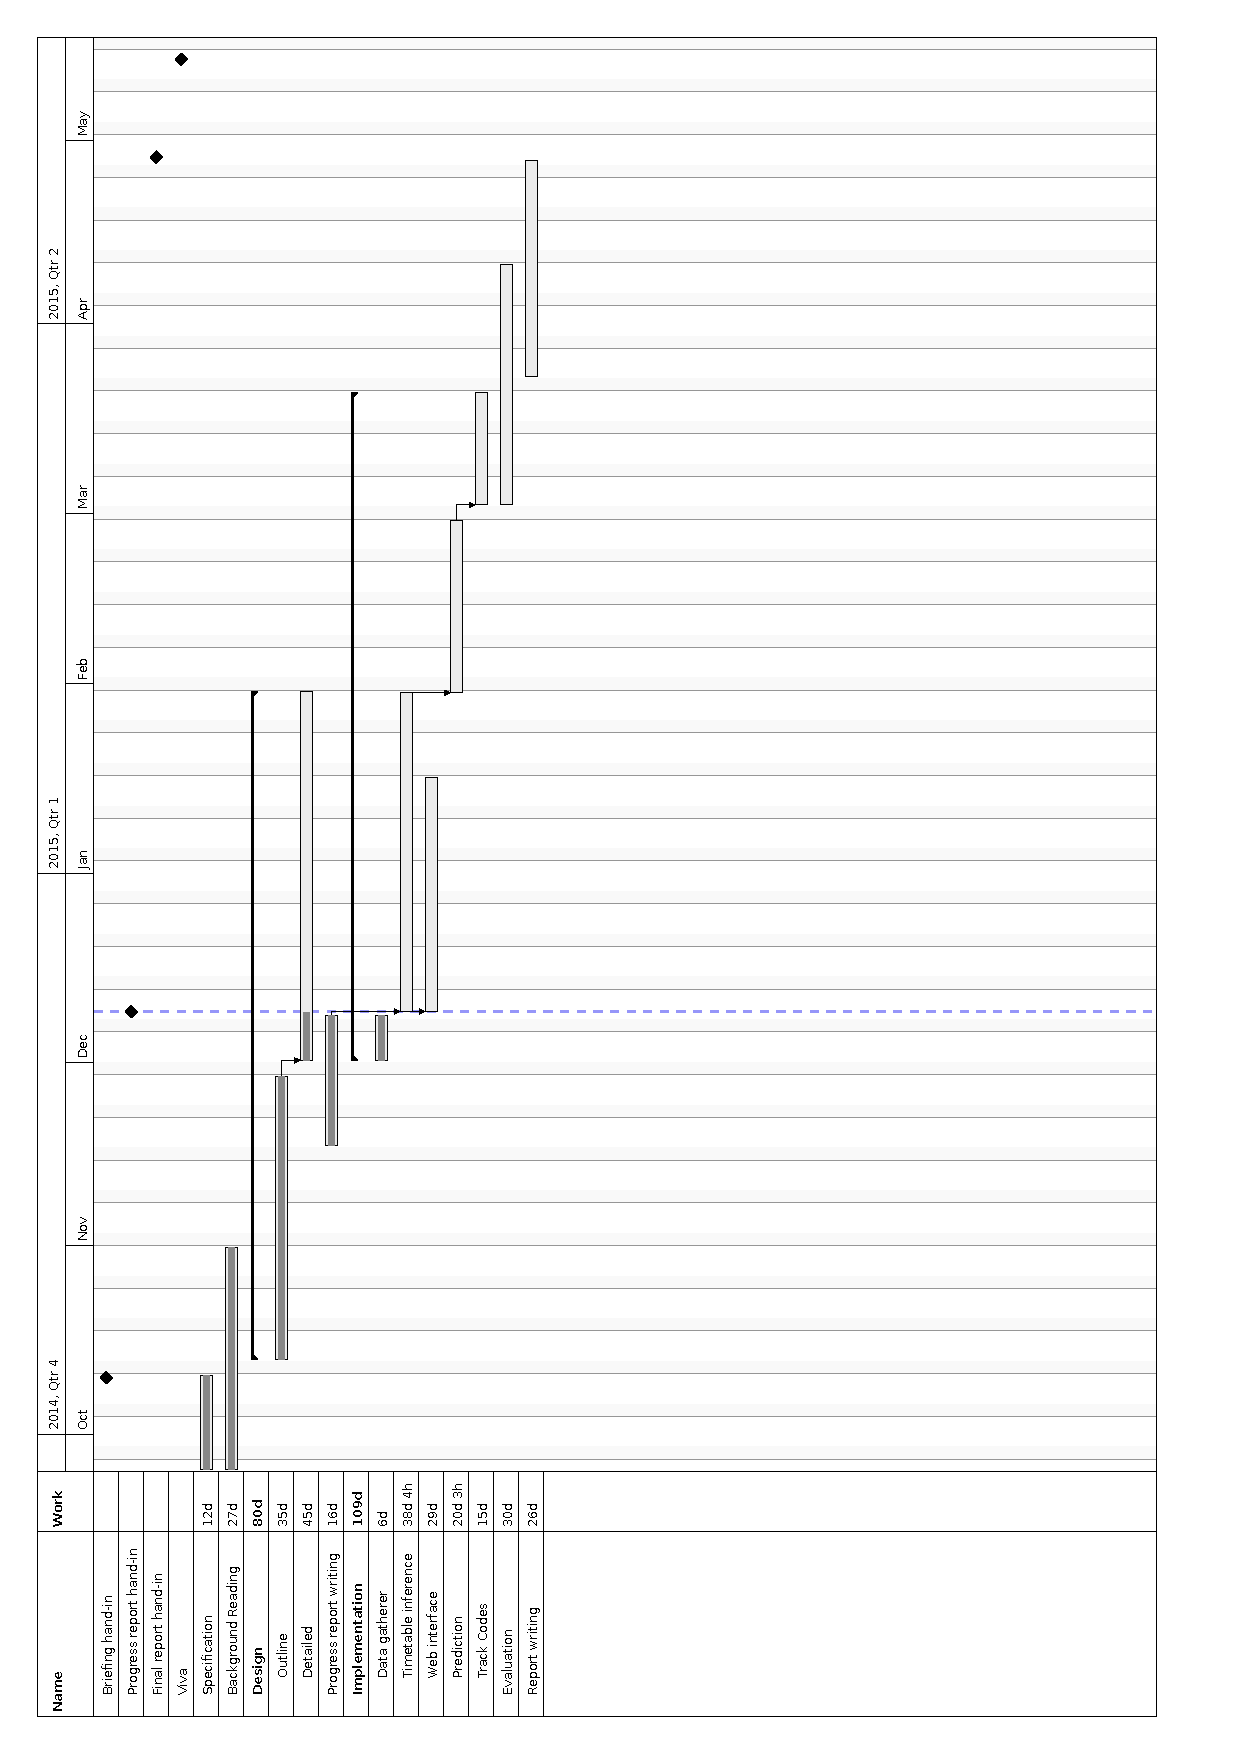
\includepdf{gantt.pdf}
\includepdf{actgantt.pdf}

\chapter{Conclusion}

This project has seen the creation of a system to continuously collect raw open
data from the London Underground and to infer from historic data a fairly
accurate timetable as well as to produce live arrival/departure times. The
system contains a web interface which allows all this data to easily be
browsed. All three main goals were fulfilled. This system is, in its current
form, probably only interesting to enthusiasts, and does not provide much more
information than existing systems. However, it lays the groundwork for either
me or future developers to improve it and add more useful functionality, or
even build entire systems around it, since it adds significant quality to the
fairly difficult to use open data provided by London Underground.

The database used in this project still contains every bit of useful
information from the source data, but has supplemented it by providing vastly
different and more useful forms with which to work, mainly live arrival and
departure times for each stop, and the inferred timetable. By these means, open
data is still available in its rawest forms should any projects require that,
but processed data can also be used where it is convenient. This appears to be
a good model for others performing processing on open data to follow.

Open data is still in its infancy, and the proliferation of sources of
unrefined, neglected or artificially restricted data is testament to this. It
should not be seen as surprising that many of these sources of data go unused
by developers for a long time, simply because of the difficulties in
transforming these data sources into a useful form. Writing this software was
much more difficult than could originally have been envisaged by anyone who had
not read the specification of TrackerNet. The major difficulties presented here
are the station-centric nature of all the data, the caching of data for 30
seconds (related to the decision to make it a pull, rather than push, service),
and the lack of useful supplementary data such as timetables and track code
maps with suitable keys for cross-referencing.

Many of these issues would not be too hard to solve through various technical
means, but as it is, the developer is left with enough data to be interesting,
but not enough to be usable without significant processing. Perhaps industries
will work past problems like this, or perhaps they will persist despite the
number of developers put off by them. In the case of the latter, more projects
such as this will be required to improve the state of open data.

This project will be made open source in due course, in order to aid the
development of future London Underground applications.

\section{Further work}

This project lays the groundwork for a system, but the stretch goals would see
that system carried to a logical next step. Firstly, a train prediction system
can be written, This would take actual times and, by cross-referencing them
with the timetable (among other things), calculate how late the train is, and
how long it will take to catch up time. Since London Underground set numbers
remain constant throughout the day, this could ``follow'' a late train's workings
to determine how long it would take for delays to be absorbed.

The next step would be to make use of track code data to build a map of track
codes, and use this map to further improve the prediction system. This would
provide even more useful data, in terms of the track code map, and would go
some way towards being able to make a live and detailed signalling map of the
system.

There are some more features that could be added to the web interface, such as
more search options, since the web interface is currently quite basic.

Finally, any other developer could pick this up and do something unexpected.

After taking a break, I might continue with these developments over the summer.

\pagebreak

\bibliographystyle{acm}

\bibliography{references}

\chapter*{Appendix A --- Sample data from TrackerNet}

\section*{PredictionDetailed}

\lstinputlisting{VUX}

\section*{LineStatus}

\lstinputlisting{LineStatus}

\section*{StationStatus}

\lstinputlisting{StationStatus}

\section*{PredictionSummary}

\lstinputlisting{V}

\chapter*{Appendix B --- Evaluation Data}

\lstinputlisting{evaluation.txt}

\end{document}
